\chapter{Implementation}

    Following the specification, the aim of this chapter is to overview aspects of the implementation stage of the proposed ALTO system.
    Firstly, attention is given to the chosen technologies that were leveraged to get the system from its specification stage into a working product - this includes tools and frameworks in the development and deployment phases, and whose choice greatly delimits the system's properties.
    Secondly, the server is put into spotlight by detailing how it is structured and how it behaves, taking special concern in how object oriented programming was leveraged to maximize modularity and reasoning of the system to facilitate future alterations and extensions.
    Special attention is given to the system's security, where an overview is made what concrete steps were taken to nullify the previously detected potential threats that put into question the viability of the system.

\section{Technologies used}

    Starting the implementation stage of every project, attention must be given into what tools are selected to make it come to fruition.
    These can greatly impact the success of the developed software, and has concrete consequence in its maintenance and future extension.

    The specified system architecture is composed by key entities whose interactions among themselves is clearly defined by interfaces.
    More so, considering the example deployment scenarios, its evident that each entity resides in different topological regions throughout the network, with then the ALTO server, clients, and status providers being scattered through an ISP domain.
    Each entity can then be thought of as a self contained system in of itself who must abide by the proposed interfaces to properly work on the system.
    A logical conclusion to this is that each entity implementation is independent from the next, needing to only assure a common communication channel that all entities within it can properly understand.
    This gives great flexibility in the system implementation as a whole, because different tools can be leveraged to different entities if needed, and such entities that be worked on independently from the rest without impacting the function of the group.

    Regarding the ALTO server, first attention is given to the ALTO resources that must be provided by it.
    They all share some common properties - such as resource id, ACLs, owner, etc. - and functionality - such as the ability to be read and updated, or their permissions modified.
    This similarity is further intensified within groups of resource types, more specifically cost maps - consider how the only concrete difference between and endpoint and a PID cost map is the type of entity the costs refer to, which are endpoint and PID addresses, respectively.
    The sequence of steps that must be taken from the initial point where a client requests a resource up until that resource is provided can be abstracted as the sequential interaction between concrete modules that have a given, self contained, purpose, and communicate with a common interface - an architectural pattern that is a micro version of the one existing in the system, that shares all its properties that were discussed previously.
    Some of these modules would include client request monitoring, its parsing, its validation, database retrieval, database storage, and serialization.
    With all this in mind, an object-oriented programming seems like a proper fit to the complexity pertaining to the ALTO server, especially considering how future extensions would be likely, as very much will be in case of the ALTO working group.
    Working with objects as the base programming entity, many of the highlighted similarities between resources will become easy to be put into evidence, and module encapsulation and interfacing are natural and thus arguably easier to develop and maintain.
    Importance is also placed in choosing a compiled language that is statically typed - a compiled language favors performance over an interpreted execution, which seems favourable for the expected scale of the ALTO system, and typed constrictions provide needed structure verifications that aid in the programmer's confidence in the program's reliability, and often reduce mistakes.
    The language choice finalizes with Java, which matches the given requirements and is the one with most prior personal development experience, coupled with its maturity and wide access to libraries and frameworks.

    The Java Spring framework is a main component of the developed server software - its inversion of control paradigm allows dependencies to be managed through configuration files and annotations to identify objects to be scanned by the framework, providing a means of development that is quite flexible, reduces boilerplate code, and favors loose coupling between objects, facilitating the independent development of implementations that can themselves be changed in the future with little consequence to the entire system, given that they implement the stipulated interface.
    Adding to this, the Spring framework provides modules that are very much needed for the server implementation, namely for MVC architectures, HTTP-based REST APIs, authentication and authorization, data access, and both unit and integration testing, to name a few.
    Given that other frameworks could provide similar functionality, Spring was favored due to its development team's focus on performance and flexibility, and because the framework has continuous development support and an increased community popularity, all of this raising the odds that this framework becomes maintained throughout the future, in comparison to some that have since lost support.

    Finally, focus was given for database decision.
    Since resource manipulation through the REST apis revolve around JSON manipulation, a preference was made for a database that allows the resources to be saved in a similar fashion, thereby reducing a layer of abstraction that makes reasoning on the software easier.
    Considering the scale at which an ALTO server might be subjected to requests, a database that favors performance seems like a better choice, in particular one that easily allows for horizontal scaling.
    A last consideration is made for a database that is schema-less - for the network information aggregation server, a myriad of types of data can be added by state providers, and more can exist in the future that weren't initially pondered by the ISP administrator, as more network protocols and data properties become relevant to attain, so a flexibility in what can be stored seems more appropriate; for the ALTO server, as the ALTO protocol itself has been subject to continuous changed that still aim for legacy support, it can be argued that future changes will be common, and doing so without increased server downtime - something that would be required by schema-driven databases - seems favorable considering the scale and importance of an ALTO service.
    The existence of private properties whose scope is outside of the protocol and can be freely defined the user, while not impossible to implement with a schema, seems to lend itself more naturally to a schema-less design.
    With all these considerations in mind, a database that abides to these constrictions and has a healthy developer support and user adoption is MongoDB, which was chosen.

    As per security, the same philosophy of the ALTO working group will be used and pre-existing, mature technologies will be leveraged.
    Hypertext Transfer Protocol Secure (HTTPS) will be used over base HTTP as a communication protocol between entities as a means to resolve many of the identified threats - by using certificates with HTTPS, the server entity authentication can be assured, and through the usage of the Transport Layer Security (TLS) as a cryptographic security tool, both confidentiality and integrity are secured via data encryption and digest calculation, respectively.
    As per client authentication, a deliberate choice was made to use HTTP basic \cite{http-basic}, as opposed to HTTP digest \cite{http-digest} that is demanded by the base ALTO working group's specification.
    With basic authentication, user and password fields are sent in encoded - not encrypted - fashion, and such information is firstly validated by the server that, if the attempt successful, proceeds with its normal operation.
    Due to the lack of encryption, this method of client authentication will be complemented with the usage of HTTPS to provide a secure communication channel that would otherwise be open to credential exposure and tampering.
    The working group's suggested digest method hashes the credentials by using a nonce - a number to be used only once - that was provided by the server, thus also protecting against data exposure and tampering.
    However, since HTTPS will be leveraged, there's no need to have an authentication system that does much more beyond of what HTTP basic does, therefore facilitating client applications and giving the server flexibility on how they wish to store user credentials - the basic authentication allows one to store the hash of passwords alone, whereas digest requires the storage of the hash value of "username:password:realm".
    These and other comparisons between these authentication methods are available at \cite{https://sci-hub.se/https://link.springer.com/chapter/10.1007/978-1-4302-6817-8_3}


\section{Server architecture}


    \textbf{[emphasis on single responsibility and behavior reutilization, as is expected on object oriented design]}

    The macro-level architectural diagram specified that the server's role is to serve incoming requests by clients and providers, and to interface with a database to persist resource storage.
    The server will implement a Representational state transfer (REST) interface leveraging the Hypertext Transfer Protocol (HTTP) as this pair is widely accepted and ubiquitous on the Internet, but also due to the fact that its resource-oriented interface standards fit nicely into the specified interface for ALTO server interactions, which too revolve around resource manipulation, and by adhering to proper REST designs good scalability can be achieved due to its stateless nature and potential for resource caching.
    The choice of HTTP as an application protocol fits nicely into a philosophy of leveraging existing and well proven protocols and technologies to increase the project's success, and indeed so was done to integrate authentication and encryption mechanisms.

    To accomplish this interface implementation, the internal server architecture will be, at a macro level, as shown in Figure \cite{fig:alto-server-architecture-macro}.
    This three-layered architecture consists firstly by a controller layer that intercepts communication requests, which after parsed and validated are redirected to the business layer, which in turn employs business logic to help satisfy the controller's requests, which may require a subsequent layer descent into the data layer via database queries.

    Figure \cite{fig:controller-unversioned-architecture} displays a class diagram focusing on controller classes that deal with resources that are not susceptible to version control - this includes every resource except the network map.
    As can be seen, all concrete controllers - such as an endpoint property map controller - are extensions to a generic controller class that is parametrized by its Data Transfer Object (DTO) , filter DTO, and service instances.
    This design choice was made because all controller logic that regards to resources without version control are the same, and by creating generic classes with type parametrization code reutilization is increased.
    The parametrization required by the controller is required to pass a concrete instance of the unversioned resource service generic class, which in of itself requires parametrization in resource DTO and resource filter DTO.
    By reflecting on common controller and service behaviour between all version control lacking resources, the conclusion was that working around generic classes maximizes reutilization, facilitates reasoning and decreases potential error.
    To help better visualize the result, refer to how the generic controller is implemented in \cite{lst:generic-controller}.
    To retrieve a resource, simply call the service class with or without the proper filter, depending on which method was triggered, by calling the appropriate methods that must implement the resource service interface.
    For example, an endpoint property map controller implementation simply extends the generic controller by providing the concrete DTO, filter DTO, and service implementations, as seen in \cite{lst:endpoint-property-map-controller}.

\begin{figure}[ht]
\centering
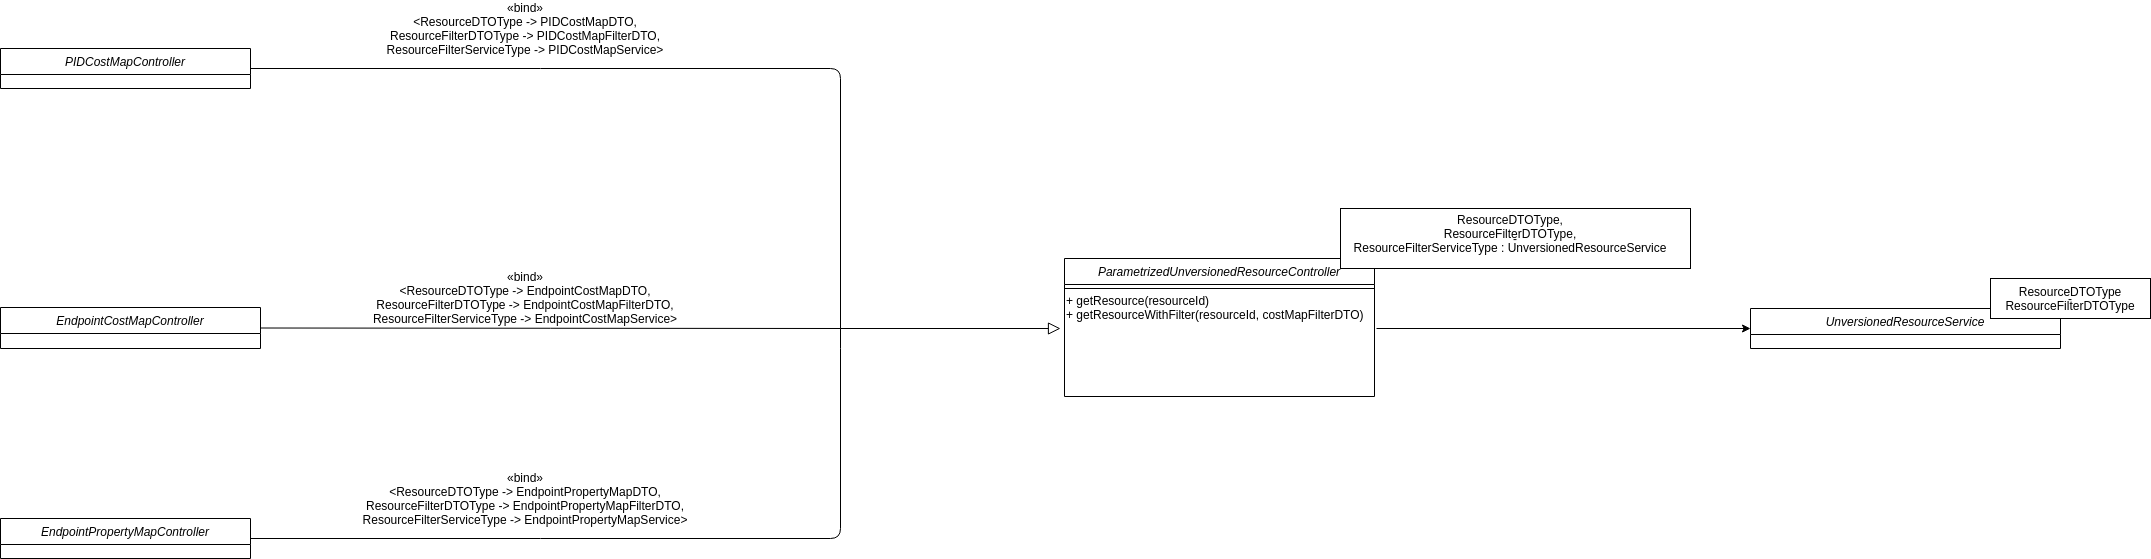
\includegraphics[scale=0.2]{img/controller-unversioned-architecture.png}
\label{fig:controller-unversioned-architecture}
\caption{Controller layer class architecture}
\end{figure}

\begin{center}
\begin{tabular}{c}
\begin{lstlisting}[caption=Parametrized Controller class for unversioned resources, label={lst:generic-unversioned-controller}]
public class ParametrizedUnversionedResourceController<ResourceDTOType,
                                                       ResourceFilterDTOType,
                                                       ResourceServiceType extends ALTOUnversionedResourceService<ResourceDTOType, ResourceFilterDTOType>> {

    private final ResourceServiceType resourceService;

    @Autowired
    public ParametrizedUnversionedResourceController(ResourceServiceType resourceService) {
        this.resourceService = resourceService;
    }

    @PreAuthorize("@ResourceAuthorizationService.hasPermission(authentication, #resourceId, T(com.example.restservice.dto.security.PermissionDTO).READ)")
    @RequestMapping(method = RequestMethod.GET, value = "{id}")
    public ResourceDTOType getResource(@PathVariable(value = "id") String resourceId) {
        return resourceService.getResource(resourceId);
    }

    @PreAuthorize("@ResourceAuthorizationService.hasPermission(authentication, #resourceId, T(com.example.restservice.dto.security.PermissionDTO).READ)")
    @RequestMapping(method = RequestMethod.POST, value = "{id}")
    public ResourceDTOType getCostMapWithFilter(@PathVariable(value = "id") String resourceId,
                                                @Valid @RequestBody ResourceFilterDTOType costMapFilterDTO) {
        return resourceService.getResource(resourceId, costMapFilterDTO);
    }
}

\end{lstlisting}
\end{tabular}
\end{center}

\begin{center}
\begin{tabular}{c}
\begin{lstlisting}[caption=Concrete controller extending from a parametrized one, label={lst:endpoint-property-map-controller}]
    @RestController
    @RequestMapping("endpointprops")
    public class EndpointPropertyMapController
        extends ParametrizedUnversionedResourceController<EndpointPropertyMapDTO, EndpointPropertyMapFilterDTO, EndpointPropertyMapService> {

        @Autowired
        public EndpointPropertyMapController(EndpointPropertyMapService resourceService) {
            super(resourceService);
        }
    }

\end{lstlisting}
\end{tabular}
\end{center}

    The same reasoning was used to implement the network map controller, but since this is the only resource that accepts versioning, the correspondent generic controller behavior does not contain similar behavior to the one above, and thus another was created, as seen in \cite{lst:versioned-controller}.
    The service layer implementation must now let the controller retrieve either a specific version of a resource, or the most recent one if no version is specified by the client.


\begin{center}
\begin{tabular}{c}
\begin{lstlisting}[caption=Parametrized controller class for versioned resources, label={lst:generic-versioned-controller}]
    public class ParametrizedVersionedResourceController<ResourceDTOType,
                                                     ResourceFilterDTOType,
                                                     ResourceServiceType extends ALTOVersionedResourceService<ResourceDTOType, ResourceFilterDTOType>> {

    private final ResourceServiceType resourceService;

    @Autowired
    public ParametrizedVersionedResourceController(ResourceServiceType resourceService) {
        this.resourceService = resourceService;
    }

    @RequestMapping(method = RequestMethod.GET, value = "{id}")
    @PreAuthorize("@ResourceAuthorizationService.hasPermission(authentication, #resourceId, T(com.example.restservice.dto.security.PermissionDTO).READ)")
    public ResourceDTOType getVersionedResource(@PathVariable(value = "id") String resourceId,
                                                @RequestParam(value = "version", required = false) String resourceVersion) {
        return resourceVersion != null
                ? resourceService.getResourceVersion(resourceId, resourceVersion)
                : resourceService.getLatestResourceVersion(resourceId);
    }

    @PreAuthorize("@ResourceAuthorizationService.hasPermission(authentication, #resourceId, T(com.example.restservice.dto.security.PermissionDTO).READ)")
    @RequestMapping(method = RequestMethod.POST, value = "{id}")
    public ResourceDTOType getVersionedResourceWithFilter(@PathVariable(value = "id") String resourceId,
                                                          @RequestParam(value="version", required = false) String resourceVersion,
                                                          @Valid @RequestBody ResourceFilterDTOType resourceFilter) {
        return resourceVersion != null
                ? resourceService.getResourceVersion(resourceId, resourceVersion, resourceFilter)
                : resourceService.getLatestResourceVersion(resourceId, resourceFilter);
        }
    }

\end{lstlisting}
\end{tabular}
\end{center}

    The purpose of some pieces of the shown code isn't immediately obvious, and will be now further explained.
    Starting with input validation, the usage of the "@Valid" annotation on an endpoint controller parameter signifies that the framework must initialize a validator class that should examine and validate that input against the defined rules.
    The rules are defined on the Data Transfer Object (DTO) class that is to be passed by the client into the server, and validation annotations from the framework are leveraged to define attribute-specific rules.
    \ref{lst:cost-map-dto}, for example, includes the "@JsonProperty" annotation that defines optional and obligatory fields in the deserialization step, and whenever needed more types of attribute validation annotations were used, including non-blank strings, non negative integers, and values within a certain non continuous set of possibilities.
    For class-wide validation, custom validator classes were created and afterwards annotated into the class in question - for the \ref{lst:cost-map-filter} class, which defines the filter DTO that is passed by the client whenever cost map filtering is selected, a custom validator class was created and annotated with "@ValidCostParametrization".
    This class, seen in \ref{lst:cost-vap-validator}, implements the class-wide restrictions imposed in the ALTO protocol regarding cost map filters, which dictate that a user can only select either a single or cost map request, and whenever calendarization is requested the total count of cost types requested must match the number of flags that dictate if a given count type must provide its calendar form.
    Assuring both attribute and class-wide rule definition and enforcement, the system can validate all user input to maintain system correctness.

    Another element from the shown controller implementation is the "@PreAuthorize" annotation.
    These, and similar others, are part of the Spring security module and serve as constriction setters that, if not successful, do not let the annotated method to execute.
    This is the basis for access control in the server system - as \ref{lst:generic-versioned-controller} shows, retrieving a resource using the GET method requires that a given constraint is verified.
    This constraint verification process is handled by a specialized created authorization service that receives authentication information, the resource id in question, and what action is being requested - in this case being "READ".
    This is how all access control restrictions upon ALTO resources is implemented - with uploaded resources containing an ACL mapping user roles to allowed actions, all controller access must first verify that the given authorized user  is authorized to perform that action.
    The authorization service, seen on \ref{lst:authorization-service}, exposes a "hasPermission" method in its interface and is tasked with confirming if the following action is allowed considering the system's constrictions and uploader's defined access control rules.
    Simply put, for a service to validate a request it must validate that the following are all true: a) the user is authenticated; b) the user has general system access to the system with that action and c) the user has concrete access to that resource with that action.
    By creating an additional access layer to the system that is separate from the resource, the server can apply both a per-role and per-resource access control, allowing more control for server administrators outside of what the resource ACLs dictate - for example, completely blacklisting a given role from a system even if a resource uploader allows him with his ACL.

    As per the service layer, a similar philosophy to the controller was taken - i.e., to expose behavior similarities and utilize generic types to inject dependency implementations.
    Listing \ref{fig:service-unversioned-architecture} displays the class diagram of services that deal with unversioned resources, and listing \ref{fig:service-versioned-architecture} shows the versioned side.

\begin{figure}[ht]
\centering
\includegraphics[scale=0.2]{img/service-unversioned-architecture.png}
\label{fig:controller-unversioned-architecture}
\caption{Unversioned service layer class architecture}
\end{figure}

\begin{figure}[ht]
\centering
\includegraphics[scale=0.2]{img/service-unversioned-architecture.png}
\label{fig:controller-unversioned-architecture}
\caption{Versioned service layer class architecture}
\end{figure}

    Much like the controller architecture, by isolating common patterns one can minimize code repetition and promote function modularity, and this results in faster development in less errors that could result in redundant logic being applied.
    As can be seen, service classes leverage resource repositories and mapper classes that translate an entity into a transfer object, which is a helpful design decision that decouples class implementation from representation, allowing the system to comply to the defined protocol without the restriction of storing and handling it the same way within the system.
    A versioned service is quite similar, but exposes an interface that lets the caller retrieve resources considering their version tag, or simply retrieve the most recent version.

    As an example, listing \ref{lst:network-map-service} shows the cost map service implementation, that simply extends the parametrized class and injects the implementations specific to how a network map service must behave - i.e., how it stores and how it translates resources.
    It then adds only methods specific to their service implementation that aren't shared among others - in this case, how to retrieve a resource with a given cost map filter, which requires different actions depending on whether or not the filter specifies a single or multi cost request.

    The mapper classes, mentioned above, are tasked with mapping between two different representations of a class.
    Specifically, mapper classes are used in the server to map between protocol representations of a resource or a filter, into representations to be used internally.
    Like previously mentioned, decoupling protocol and internal class representations makes the resources easier to store, as they can be translated into a form more ideal for MongoDB storage - in some cases making some queries quite impossible to achieve otherwise - and easier to handle, since protocol representation of data is better for data transmission and readability, but not as much for querying and algorithmically processing.
    For example, the protocol representation of calendarized cost maps separates the cost information, cost values and calendar information into three separate entities, and their matching must be made by equal index access.
    Working internally with a data structure that is optimized for simpler and quicker data handling and querying can optimize application performance and reduce code complexity, being a good compromise for the added mapping layer that is consequentially required.
    As an example, listing \ref{} display how a calendar cost map is represented in the ALTO protocol, and in comparison listing \ref{} shows that same display as a storage-ready entity.

    \todo{protocol costmap vs database costmap}

    Data access is materialized in the form of repository classes, responsible for providing an interface for service classes that let them retrieve entity classes from the database, doing so by generating the required queries to the Mongo database.
    Again, for behaviour similarity exposure, the repositories inherit from a base versioned and unversioned repository that compiles the queries needed to retrieve resources, requiring the inheriting repositories to specify additional implementation-specific queries needed to extend upon the functionality.
    For this to be possible, entity representation on the database must too be similar, so the base queries, when applied to either a network map or an endpoint property map, two unversioned example resources, can work the same.
    Listing \ref{} and \ref{} show an example database representation of a cost map and an endpoint, respectively.
    Notice how common properties are indexed in the same way, and only differ on implementation-specific details.
    The "resourceId" attribute can be queried and the "mappingEntities" attribute can be loaded by the high-level query without needing to know what concrete resource entity is being treated, and further implementation-specific querying is made by the inheriting repositories.

    \todo{database cost map vs endpoint property map}

    Listing \ref{} shows a portion of the network map repository implementation.
    To retrieve a specific version of a resource, build query methods are retrieved from the versioned repository class, and network map specific processing is added to apply network map projections - which in this case means retrieving only the specified pids.

    A good API must be aware of possible errors that may occur, and communicate these to the client in a way that is easy to understand.
    To achieve this, a global exception handling mechanism was used with the aid of the "@RestControllerAdvice" annotation, that is tagged to a class that will consequently catch and process controller-thrown exceptions, which themselves could've been propagated from the service, mapper, or repository layers.
    It then centralizes the error handling aspect that is then focused in building the correct error packets that contain the appropriate HTTP code and a message with helpful details.
    These message details are extracted directly from the thrown exception, but it is important to assume that these are to be exposed to the clients, and thus should not contain heavy implementation details for developers, with logging instead taking that role.
    Listing \ref{} shows the main exception handler used.


\section{Network information aggregator}

    \textbf{[How the network information aggregator server was implemented to receive network measurements - interface, validation, security, etc. Will be similar to the ALTO server with the difference that it handles measurement collection instead of ALTO resources collection]}

\section{Network state providers}

    \textbf{[Overviews the implementation of some of the network state providers developed - one listens for OSPF messages, another reads csv files, etc, and all upload to the interface implemented by the network information aggregator]}

\section{Server discovery}
    \textbf{[Leveraging DNS like the working group suggests]}

